\chapter{Implementation}

\label{Chapter4}

\lhead{Chapter 4. \emph{Implementation}}

In this chapter, a comprehensive overview of the libraries utilized throughout and the functions applied for 
achieving topic modelling, specifying their roles in different sections of the code is given. Through deeper 
understanding of the inner workings od modelling and explaining the implementation of the algorithms, the thesis is concluded.

For implementation of the thesis, I have used platform like VS Code(Visual Studio Code) and Jupyter Notebook(Jupyter Notebook).
VS code is integrated developement environment and Jupyter Notebook is a web based IDE, where both this IDE will support various 
languages and frameworks for the model implementation and developement.

%%%%%%%%%% Librarues %%%%%%%%%%%
\section{Libraries}

In this section, we will focus on certain aspects of libraries and their uses in the model implementation process.

%%%%%%%%%% Pandas %%%%%%%%%%%
\noindent\textbf{Pandas:}

Pandas is a library that is commonly used for data analysis and manipulation. It provides different functions and methods that are compatible with 
structured data such as data frames, CSV files, Excel sheets, etc. This library is very helpful in projects related to data science, 
machine learning and data analytics because it facilitates tasks such as: data cleaning; pre-processing; manipulation; visualization among others. \cite{pythonlibrary}.


%%%%%%%%%% NumPy %%%%%%%%%%%

\noindent\textbf{NumPy:}

NumPy is a fundamental package for scientific computing in the python which provides a multidimensional array object, 
derived object (like masked array and matrices) and an assortment of routines for fast operations on arrays which 
includes mathematical, logical, shape manipulation, sorting, selecting, I/O, discrete Fourier transforms, basic algebra,
 statistical operations, and much more. NumPy have been used in few places in this thesis, like converting the 
 embedded data into an array so that it can be used for dimensional reduction and to find
the total number of clusters formed \cite{pythonlibrary}.

%%%%%%%%%% Pickle %%%%%%%%%%%
\noindent\textbf{Pickle:}

 Pickle is one of the most used libraries in python for data serialization and deserialization as it converts objects 
 into bytes streams for storage and restore them into original form. As pickle can handles objects of python includes 
 list, dictionaries and so on, using different protocols optimized for efficiency. Common use cases include saving 
 objects states, caching, and inter-process communication. The pickle library is used to store the embedded data 
 formed as the data set is huge and running embedding every time takes lot of time \cite{pythonlibrary}.

  %%%%%%%%%% Json %%%%%%%%%%%
\noindent\textbf{Json:}

The python json module will offers a means of encoding and decoding data in the lightweight, text-based JSON (Javascript Object Notation)
format which is frequently used for data transmission. The module allows you to serialize python objects, 
such as dictionaries, lists into json strings and deserialize json strings into python objects. Json is a human readable 
and language independent which can be used for web APIs and configuration files. Json format is used for storing the 
clustered data as this format is human readable and can be used for APIs as the clustered data will be feeded into the 
large language model \cite{pythonlibrary}.

 %%%%%%%%%% umap-learn %%%%%%%%%%%
\noindent\textbf{umap-learn:}

umap-learn is an open-source python package will helps to implement the Uniform Manifold Approximation and Projection 
algorithm for dimensionality reduction. It does this by first learning a high-dimensional graph representation of 
the data, and thereafter, optimizes a low-dimensional layout which captures the local structure. 
The umap-learn package offers an easy-to-use interface, in addition to native interfaces to other 
well-known data science libraries like Pandas, Scikit-learn, and NumPy. It can also deal with supervised and 
unsupervised learning, which turns out to be versatile for many applications. Of these, a very notable one is 
dimensionality reduction of feature spaces, hence improving efficiency to downstream tasks like data visualization, 
classification or clustering \cite{pythonlibrary}. 
\vspace{2cm}
%%%%%%%%%% hdbscan %%%%%%%%%%%

\noindent\textbf{hdbscan:}

hdbscan is a Python package that implements the HDBSCAN (Hierarchical Density-Based Spatial Clustering 
of Applications with Noise) algorithm. This package is often used in tasks which involves complex data
 like biology, image processing, grouping the text etc., and this can be easily integrated with the other
  libraries like Pandas and scikit-learn. This algorithm is used for discovering the patterns in large 
  dataset where number of clusters is unknown \cite{pythonlibrary}.

%%%%%%%%%% transformers %%%%%%%%%%%
\noindent\textbf{transformers:}

The transformers package is by Hugging Face is a powerful library that allows to access the wide range if pretrained transformers models for many NLP tasks. It supports both PyTorch and 
TensorFlow and it is easy to use where APIs allows the user to load the models. tokenize data and fine tune them. The package also includes a convenient pipeline API for applying models 
to various tasks with minimal code. With extensive documentation and a large community, transformers has become a go-to tool for state-of-the-art NLP \cite{pythonlibrary}.

%%%%%%%%%% torch %%%%%%%%%%%
\noindent\textbf{torch:}

 Troch is a deep learning library that is used for machine learning, and it is core library of PyTorch, a popular open source framework developed by Facebook's AI research lab. PyTorch is widely used 
 for building and training deep learning models due to its speed, flexibility, and ease of use. This package provides a range of functionalities, including tensor operations (Similar to Numpy arrays with 
 GPU acceleration), automatic differentiation, and building neural networks. It also supports GPU acceleration using CUDA, making it suitable for high-performance computing \cite{pythonlibrary}.

\noindent\textbf{Flask:}

Flask, being an adaptable and simple web framework helps to create web apps with python.
the server-side processing is handled via this tool while it also influences the web request
management thanks to its essential utility for forming a web server and directing the requests
between the front-end and back-end section of the application \cite{pythonlibrary}. 
\vspace{1cm}

\noindent\textbf{HTML/CSS:}

The application's front-end was developed with HTML for structure and CSS for styling. This combination ensures the user interface is functional and attractive.
Hence, it is able to carry out its task without much ado and in a commendable way as well. User input is collected using HTML forms while CSS serves the purpose of improving on webpage aesthetics.


%%%%%%%%%% Code Implementation %%%%%%%%%%%

\section{Code Implementation}

This section will explain how the code is implemented in the thesis to achieve topic modelling. 
This section consist of subsection as follows:
\begin{enumerate}
  \item Preprocessing
  \item Embedding
  \item Dimensionality reduction
  \item Clustering
  \item Large Language Model
\end{enumerate}

%%%%%%%%%% Preprocessing %%%%%%%%%%%

\subsection{Preprocessing}

Once the initial data analysis has been done, the data will undergoes preprocessing steps as mentioned below,
%%%%%%%%%%%% code %%%%%%%%%%%
\begin{lstlisting}[language=Python , caption={Initialization of the list of noise}]
# List of common filler words
filler_words = {"ja", "hm", "mhm", "ach", "gut", "und", "eben", "ne", "ok", "aha", "ach so", "nicht", "ja", "nein", "wieder", "schon", "naja", "wieso", "wieso nicht", "wieso nicht"}

\end{lstlisting}

As there the data is the transcript of the video Interviews, it consists of lot noise in the data. There are lot of shot sentence, noise, repeated small sentences etc., hence, it is necessary to remove them.
The below code has list of noise which can be removed from the data. and this is the initialization of the list.
%%%%%%%%%%% code %%%%%%%%%%%

\begin{lstlisting}[language=Python, caption={Filtering of noise from the data}]
  def has_repeated_filler_patterns(sentence, filler_words):
    # Check if any filler word appears repeatedly either consecutively or separated by commas or spaces in the sentence.
      pattern = r'\b(' + '|'.join(re.escape(word) for word in filler_words) + r')\b(?:[\s,]+)+\1\b'
      
      if re.search(pattern, sentence):
          return True
      return False
  \end{lstlisting}

 
  The function \texttt{has\_repeated\_filler\_patterns} is useful when talking about text because it helps by filtering out certain sentences from it while breaking the text down into different sentences through regular
   expressions that look for punctuation marks showing end of sentence. This function checks a variety of factors including minimum word count as well as unique word count. If all these conditions are met, 
   then that particular sentence will go into a filtered sentence list. In addition this could also call has repeated filler patterns to eliminate noise.
%%%%%%%%%%% code %%%%%%%%%%%
\begin{lstlisting}[language=Python, caption={Filter sentences from the text}]
def filter_short_and_filler_sentences(text, filler_words, min_words, min_unique_words, min_characters):
    # Filter sentences from the text based on length, unique words, minimum characters, and absence of repeated filler patterns.
    sentences = text.split('. ')
    filtered_sentences = []

    for sentence in sentences:
        words = sentence.split()
        
        if len(words) >= min_words and len(set(words)) >= min_unique_words and len(sentence) >= min_characters:
            if not has_repeated_filler_patterns(sentence, filler_words):
                filtered_sentences.append(sentence)
    
    return '. '.join(filtered_sentences)
\end{lstlisting}

The \texttt{filter\_short\_and\_filler\_sentences} function will process the text to filter out sentences and it splits the text into individual sentences using the regular expression to check the various
punctuation marks that signify the end of a sentence. This function check several conditions like minimum number of words number of unique words and exceed the length in characters once these conditions are satisfied, 
the sentence will be appended to the list of filtered sentences. 
Additionally, it will call \texttt{has\_repeated\_filler\_patterns} function to identify and remove noise.
\vspace{3cm}

%%%%%% code %%%%%%%
\begin{lstlisting}[language=Python, caption={Removing columns and combining the sentences to paragraphs}]

    excel_data = pd.read_excel(file_path, sheet_name=None)

    # Combining the sentences to paragraphs and applying the filtering
    combined_paragraphs = {}
    
    for sheet_name, df in excel_data.items():
        # Drop the 'Timecode' and 'Sprecher' columns
        df = df.drop(columns=['Timecode', 'Sprecher'])
        
        # Convert the 'Transkript' column to a single string
        df['Transkript'] = df['Transkript'].astype(str)
        paragraph = ' '.join(df['Transkript'].tolist())
        
        # Filter short sentences and apply filler pattern filtering
        filtered_paragraph = filter_short_and_filler_sentences(paragraph, filler_words, min_words, min_unique_words, min_characters)
        
        # Save the filtered paragraph by sheet name in the dictionary
        combined_paragraphs[sheet_name] = filtered_paragraph
    
    # The `combined_paragraphs` dictionary now contains the filtered paragraphs for each sheet in memory.
    # You can now use `combined_paragraphs` as needed in your code.
    
    print("Filtered paragraphs have been processed and stored in memory.")
        
\end{lstlisting}

The above code will help to read the excel file, remove the columns and combine the sentences to paragraphs, where it reads the data from each sheet in the excel file and removes the columns Timecode and Sprecher. 
It also combines the data into one single paragraph by adding the sheet name to the start of the paragraph. This code will call the \texttt{filter\_short\_and\_filler\_sentences} function
 to filter the sentences and adds the sheet name at the begin of the paragraph and save the 
combined data to a text file and pickle file for the future use.

%%%%%%%%%% Embedding %%%%%%%%%%%

\subsection{Embedding}
 This the code will load the pre-trained Jina embeddings model and tokenizer the pre-processed text data. 
 The model will be used convert the text data into embeddings.

%%%%%% code %%%%%%%
 \begin{lstlisting}[language=Python, caption={Load Jina AI embedding model and tokenizer}]

# Load the pre-trained Jina embeddings model and tokenizer
model_name = 'jinaai/jina-embeddings-v2-base-de'
model = AutoModel.from_pretrained(model_name, trust_remote_code=True)
tokenizer = AutoTokenizer.from_pretrained(model_name, trust_remote_code=True)

# Assigning the combined_paragraphs to the text variable
text = combined_paragraphs
# Split the text into sentences based on '. ' delimiter
sentences = text.split('. ')
# Define the batch size for processing
batch_size = 32 # can be adjusted based on the computational power
embeddings = []

# Process the sentences in batches
for i in range(0, len(sentences), batch_size):
    batch_sentences = sentences[i:i+batch_size]
    
    # Tokenize the batch of sentences
    inputs = tokenizer(batch_sentences, return_tensors='pt', padding=True, truncation=True, max_length=512)
    # Compute embeddings without tracking gradients
    with torch.no_grad():
        outputs = model(**inputs).last_hidden_state
        
        # Compute the mean embedding for each sentence in the batch
        batch_embeddings = outputs.mean(dim=1).cpu().numpy()
        # Append the batch embeddings to the list
        embeddings.extend(batch_embeddings)

# Convert the list of embeddings to a NumPy array
embeddings = np.array(embeddings)
\end{lstlisting}

\noindent\textbf{Load Model and Tokenizer:} It loads a pre-trained Jina embeddings model and its corresponding tokenizer. 
The \texttt{trust\_remote\_code=True} argument ensures that remote code is trusted when loading the model.

\noindent\textbf{Split Text:} The data is split into individual sentences using '. ' as the delimiter.
As the text dataset has been combined into a paragraph, it is necessary to split the text into individual sentences.
As the model can handle sequences length of the embeddings is 8192 and I have reduced to sequence length to 512 as in the future phase
as the maximum sequence length need more computational power and memory. 

\noindent\textbf{Batch Processing:} Sentences are processed in batches of size 32 to manage memory and computational efficiency.
This will also reduces the runtime of the embedding process. The batch size can be alter based on the computational power.

\noindent\textbf{Tokenization and Embedding Computation:} Each batch of sentences is tokenized using the model’s tokenizer. 
The embeddings are computed without tracking gradients for efficiency. For every sentence, a fixed size embedding is 
obtained by calculating the mean of the last concealed state across tokens.

\noindent\textbf{Store Embeddings:} The embeddings for each batch are collected and converted into a NumPy array for further use.

%%%%%%%%%% Dimensionality Reduction %%%%%%%%%%%%%

\subsection{Dimensionality Reduction}

As the embedding data will be having high dimensional space and it cannot be used for the visualization and clustering directly hence, the UMAP reduction
technique is used which will helps to convert the high dimensional space into a low dimensional space.

%%%%%% code %%%%%%%
\begin{lstlisting}[{language=Python, caption={Dimensionality Reduction}}]
import umap.umap_ as umap
# Create a UMAP model instance with specified hyperparameters
umap_model = umap.UMAP(n_neighbors=20, n_components=10, min_dist=0.1, metric='cosine', low_memory=True)

# Fit the UMAP model to the filtered embeddings and transform the data
umap_embeddings = umap_model.fit_transform(filtered_embeddings)
\end{lstlisting}

\noindent\textbf{Initialize UMAP Model:} The UMAP model is initialized with the following hyperparameters:
\begin{itemize}
    \item \texttt{n\_neighbors}: Number of neighboring points used in local approximations.
    \item \texttt{n\_components}: The number of dimensions for the reduced embedding.
    \item \texttt{min\_dist}: Minimum distance between points in the low-dimensional space.
    \item \texttt{metric}: Distance metric used to calculate distances between points.
    \item \texttt{low\_memory}: Optimizes memory usage by storing fewer intermediate results.
\end{itemize}
These hyperparameters will help to balance capturing both local and  global structure in the data while reducing the dimension of the data. Setting the \texttt{n\_neighbors}
will allows the model to consider neighborhood size preserving both local relationships and broder patterns. The \texttt{n\_components} which will helps to retains the 
important information for downstream tasks with any data loss. The \texttt{min\_dist} will relatively control the distance between groups and tightens the clusters making it easier for 
grouping the distinct groups. The use of \texttt{low\_memory=True} will help to reduce the memory usage of the model whenever it is dealing with larger dataset.

\noindent\textbf{Fit and Transform Data:} The UMAP model is trained on the \texttt{filtered\_embeddings} data to reduce its dimensionality from high-dimensional space to a 10-dimensional space. 
The \texttt{fit\_transform()} method performs both fitting the model and transforming the data into the new lower-dimensional space. The transformed data is stored in \texttt{umap\_embeddings}.

%%%%%%%%%% Clustering %%%%%%%%%%%%%

\subsection{Clustering}
HDBSCAN is used to cluster the embeddings obtained from UMAP. The clustering results are organized into a JSON file 
to facilitate easy access and analysis of the clusters and their associated sentences.


%%%%%% code %%%%%%%
\begin{lstlisting}[{language=Python, caption={HDBSCAN Clustering}}]

# Create a HDBSCAN Clustering instance with specified hyperparameters
clusterer = hdbscan.HDBSCAN(min_cluster_size=40, cluster_selection_epsilon=0.4, metric='euclidean', cluster_selection_method='eom')
clusters = clusterer.fit_predict(umap_embeddings)

# Print the number of clusters
num_clusters = len(set(clusters)) - (1 if -1 in clusters else 0)
print(f"Number of clusters: {num_clusters}")
\end{lstlisting}

\noindent\textbf{Initialize and Apply HDBSCAN:} The HDBSCAN clusterer is configured with:
\begin{itemize}
    \item \texttt{min\_cluster\_size}: Minimum size of clusters.
    \item \texttt{cluster\_selection\_epsilon}: The parameter to regulate the clusters granularity.
    \item \texttt{metric=}: The distance metric used for clustering.
    \item \texttt{cluster\_selection\_method}: Method for selecting clusters (excess of mass).
\end{itemize}
The \texttt{fit\_predict()} method applies HDBSCAN to the \texttt{umap\_embeddings} and returns cluster labels.

\noindent\textbf{Count and Print Number of Clusters:} The number of clusters is calculated by counting unique cluster labels and adjusting for the label \texttt{-1},
 which represents noise. The result is printed.
\vspace{3cm}

%%%%%% code %%%%%%%
\begin{lstlisting}[{language=Python, caption={Count and Print Number of Clusters}}]
# Create a list to hold clusters with their sentences
clusters_list = []

for cluster in np.unique(clusters):
    # Convert the cluster ID to a regular Python int
    cluster_id = int(cluster)
    # Collect sentences for each cluster
    sentences_in_cluster = [sentence for i, sentence in enumerate(sentences) if clusters[i] == cluster]
    
    # Create a dictionary for the cluster
    cluster_dict = {
        "cluster_id": cluster_id,
        "sentences": sentences_in_cluster
        }
    # Add the cluster dictionary to the list
    clusters_list.append(cluster_dict)
    
# Save the clusters to a JSON file
output_json_file = 'clusters.json'
with open(output_json_file, 'w', encoding='utf-8') as f:
    json.dump(clusters_list, f, ensure_ascii=False, indent=4)

print(f"Clusters have been saved to '{output_json_file}'")
\end{lstlisting}

\noindent\textbf{Organize and Store Clusters:} The code creates a list of dictionaries where each dictionary represents a cluster. Each dictionary contains:
\begin{itemize}
    \item \texttt{cluster\_id}: The ID of the cluster.
    \item \texttt{sentences}: A list of sentences belonging to that cluster.
\end{itemize}

\noindent\textbf{Save Clusters to JSON:} The list of clusters is saved to a JSON file named \texttt{clusters.json}. 
The \texttt{json.dump()} function serializes the list and writes it to the file. A confirmation message is printed indicating successful saving.


%%%%%%%%%%%%%%%% large Language Model %%%%%%%%%%%%%%%%

\subsection{Large Language Model}

The cluster data which is stored in the JSON file is used to generate the topic names for each cluster. This process involves leveraging the model’s ability to process and synthesize information from multiple sentences,
producing a coherent and meaningful topic label for each cluster.

\noindent\textbf{Loading the Model and Tokenizer:} Accessing the pre-trained language model and tokenizer through Hugging 
Face model hub with a script that has a name Meta-Llama-version, it is based on an 
access token (this model is being used because of my compute resources constraints although other models may be possible too).
%%%%%% code %%%%%%%
\begin{lstlisting}[{language=Python, caption={Loading Llama 3 model}}]
import json
import torch
from transformers import AutoModelForCausalLM, AutoTokenizer

# Debugging function to help track where issues might be occurring
def debug_message(message):
    print(f"[DEBUG] {message}")
# Load the model and tokenizer once at the beginning
try:
    debug_message("Loading model and tokenizer...")
    model = AutoModelForCausalLM.from_pretrained("meta-llama/Meta-Llama-3-8B", token="HuggingFace access token")
    tokenizer = AutoTokenizer.from_pretrained("meta-llama/Meta-Llama-3-8B", token="HuggingFace access token")
    debug_message("Model and tokenizer loaded successfully.")
except Exception as e:
    debug_message(f"Error loading model or tokenizer: {str(e)}")
    raise
\end{lstlisting}

\noindent\textbf{Generating Topics:} A function named \texttt{generate\_topic} is used to generate a topic name for a set
 of sentences within a cluster. The sentences are combined into a corpus and fed to the language model using a prompt,
  which returns a concise and specific topic of up to 5 words. 
The topic generation process is wrapped in error handling to catch any issues that may arise. 
%%%%%% code %%%%%%%
\begin{lstlisting}[{language=Python, caption={Generate Topic}}]
def generate_topic(sentences):
    try:
        # Combine sentences into a single string
        combined_sentences = " ".join(sentences)  
        # Create a prompt for the model
        prompt = f"Analysiere die folgenden Saetze und generiere einen praezisen, aussagekraeftigen Themennamen von maximal 5 Worten. Der Themenname sollte den Kerninhalt erfassen und spezifisch sein. Saetze: {combined_sentences} Thema:"
        # Tokenize input and generate the topic
        inputs = tokenizer(prompt, return_tensors="pt")
        outputs = model.generate(**inputs, max_new_tokens=10, num_return_sequences=1)
        # Decode the generated topic
        return tokenizer.decode(outputs[0], skip_special_tokens=True).strip()
            
    except Exception as e:
        debug_message(f"Error during topic generation: {str(e)}")
    return "Topic generation failed"
\end{lstlisting}

\noindent\textbf{Loading Clusters:} The clusters of sentences are loaded from a JSON file (\texttt{clusters.json}), 
which contains a list of dictionaries. Each dictionary represents a cluster and includes a \texttt{cluster\_id} 
and the corresponding \texttt{sentences}.
%%%%%% code %%%%%%%
\begin{lstlisting}[{language=Python, caption={Load Clusters from JSON}}]
# Load the clusters from the JSON file
input_json_file = 'clusters.json'
try:
    debug_message(f"Loading clusters from {input_json_file}...")
    with open(input_json_file, 'r', encoding='utf-8') as f:
        clusters_list = json.load(f)
    debug_message("Clusters loaded successfully.")
except Exception as e:
    debug_message(f"Error loading clusters: {str(e)}")
    raise

# List to hold the results with generated topics
clusters_with_topics = []
\end{lstlisting}

\noindent\textbf{Processing Clusters Sequentially:} The function \texttt{process\_clusters\_sequentially} iterates through
 each cluster, skipping any noise clusters (identified by \texttt{cluster\_id} = -1). For each valid cluster, 
the function generates a topic, appends the topic to the cluster data, and adds the updated cluster to a list 
(\texttt{clusters\_with\_topics}). After processing each cluster, the script clears the CUDA memory (if using a GPU)
 to optimize memory usage.
%%%%%% code %%%%%%%
\begin{lstlisting}[{language=Python, caption={Process Clusters Sequentially}}]
def process_clusters_sequentially():
    for cluster in clusters_list:
        try:
            # Extract cluster information
            cluster_id = cluster["cluster_id"]
            # Skip the cluster with ID -1 (noise)
            if cluster_id == -1:
                debug_message(f"Skipping noise cluster {cluster_id}")
                continue
            
            sentences = cluster["sentences"]
            # Debug: Show the cluster info
            debug_message(f"Processing cluster {cluster_id} with {len(sentences)} sentences.")
            
            # Generate a topic for the cluster
            topic = generate_topic(sentences)
            # Add the generated topic to the cluster data
            cluster["topic"] = topic
            # Append the updated cluster to the results list
            clusters_with_topics.append(cluster)
            # Clear memory after processing each cluster
            torch.cuda.empty_cache()  # If you're using a GPU, clear the cache
            debug_message(f"Processed cluster {cluster_id}, Topic: {topic}")        
        except Exception as e:
            debug_message(f"An error occurred while processing cluster {cluster_id}: {str(e)}")

# Process all clusters sequentially
try:
    process_clusters_sequentially()
except Exception as e:
    debug_message(f"Error during cluster processing: {str(e)}")
    raise
\end{lstlisting}

\noindent\textbf{Saving Results:} Once all clusters have been processed, the updated clusters with generated topics 
are saved to a new JSON file (\texttt{clusters\_with\_topics.json}) for further use.
%%%%%% code %%%%%%%
\begin{lstlisting}[{language=Python, caption={Save Clusters with Topics to JSON}}]  
# Save the clusters with topics to a new JSON file
output_json_file = 'clusters_with_topics.json'
try:
    debug_message(f"Saving clusters with topics to {output_json_file}...")
    with open(output_json_file, 'w', encoding='utf-8') as f:
        json.dump(clusters_with_topics, f, ensure_ascii=False, indent=4)
    debug_message("Clusters with topics saved successfully.")
except Exception as e:
    debug_message(f"Error saving clusters: {str(e)}")
    
\end{lstlisting}
Throughout this code, a debugging function (\texttt{debug\_message}) is used to print out messages for tracking the 
progress and identifying potential issues.

\vspace{5cm}
% |---------------------------------------------------------------------------------|
% Application for the smaller text
% |--------------------------------------------------------------------------------|

\section{Web Application for Smaller Text Corpus}

In this section, the development of the a web application designed to process the smaller text data with the above implementation.
The primary goal of this application is to provide a user-friendly interface for analysis of the smaller text corpus. This application
will also the same workflow but, the data will be directly feed into the embedding model which is followed by clustering then to the 
LLM model (Llama).

\subsection{Methodlogy and Technologies Used}
To implement this web application the following Technologies are employed, I have used the function which i have used in 
the previous section along with the flask and HTML/CSS. Here the flask is used to run the web application where is manage the 
POST request and Get request. The HTML/CSS is used to design the user interface (UI). The data is processed in the same way 
as in the previous section.
Over here instead of loading the files the user can directly paste the text data which we want to do topic modelling. 
Once the data is loaded then the user can change the minimum size of the cluster and click on process button to process the data. 
The data will be undergo the same process which is mwntion in thw previous section like embedding, clustering and then
to language model to generating the topic. 

\noindent Below are few snapshots of the web application, 

This is the UI of the web application where the user can change the minimum size of the cluster and process the data.
\begin{figure}[htbp]
    \begin{center}
      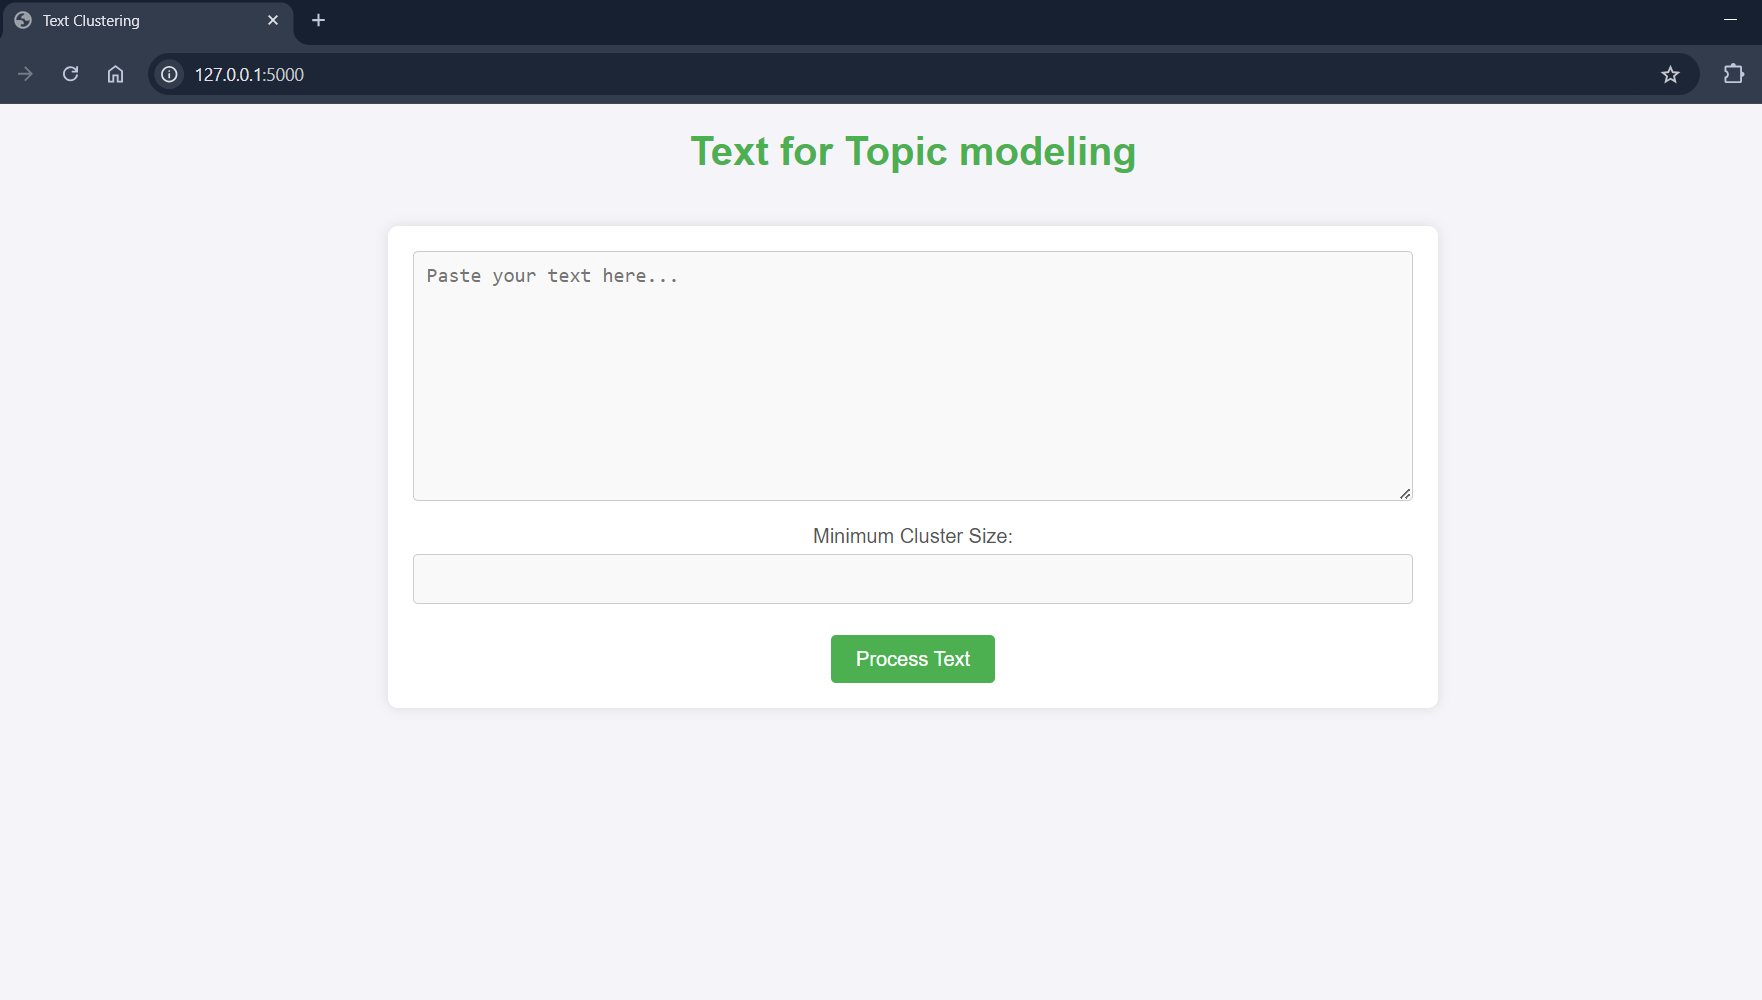
\includegraphics[width=12cm]{./Images/UI 1.png}
       \caption{UI for the web application}
       \label{fig: Web application UI}
    \end{center}
\end{figure}

The output of the web application looks as attached below,

\begin{figure}[htbp]
    \begin{center}
      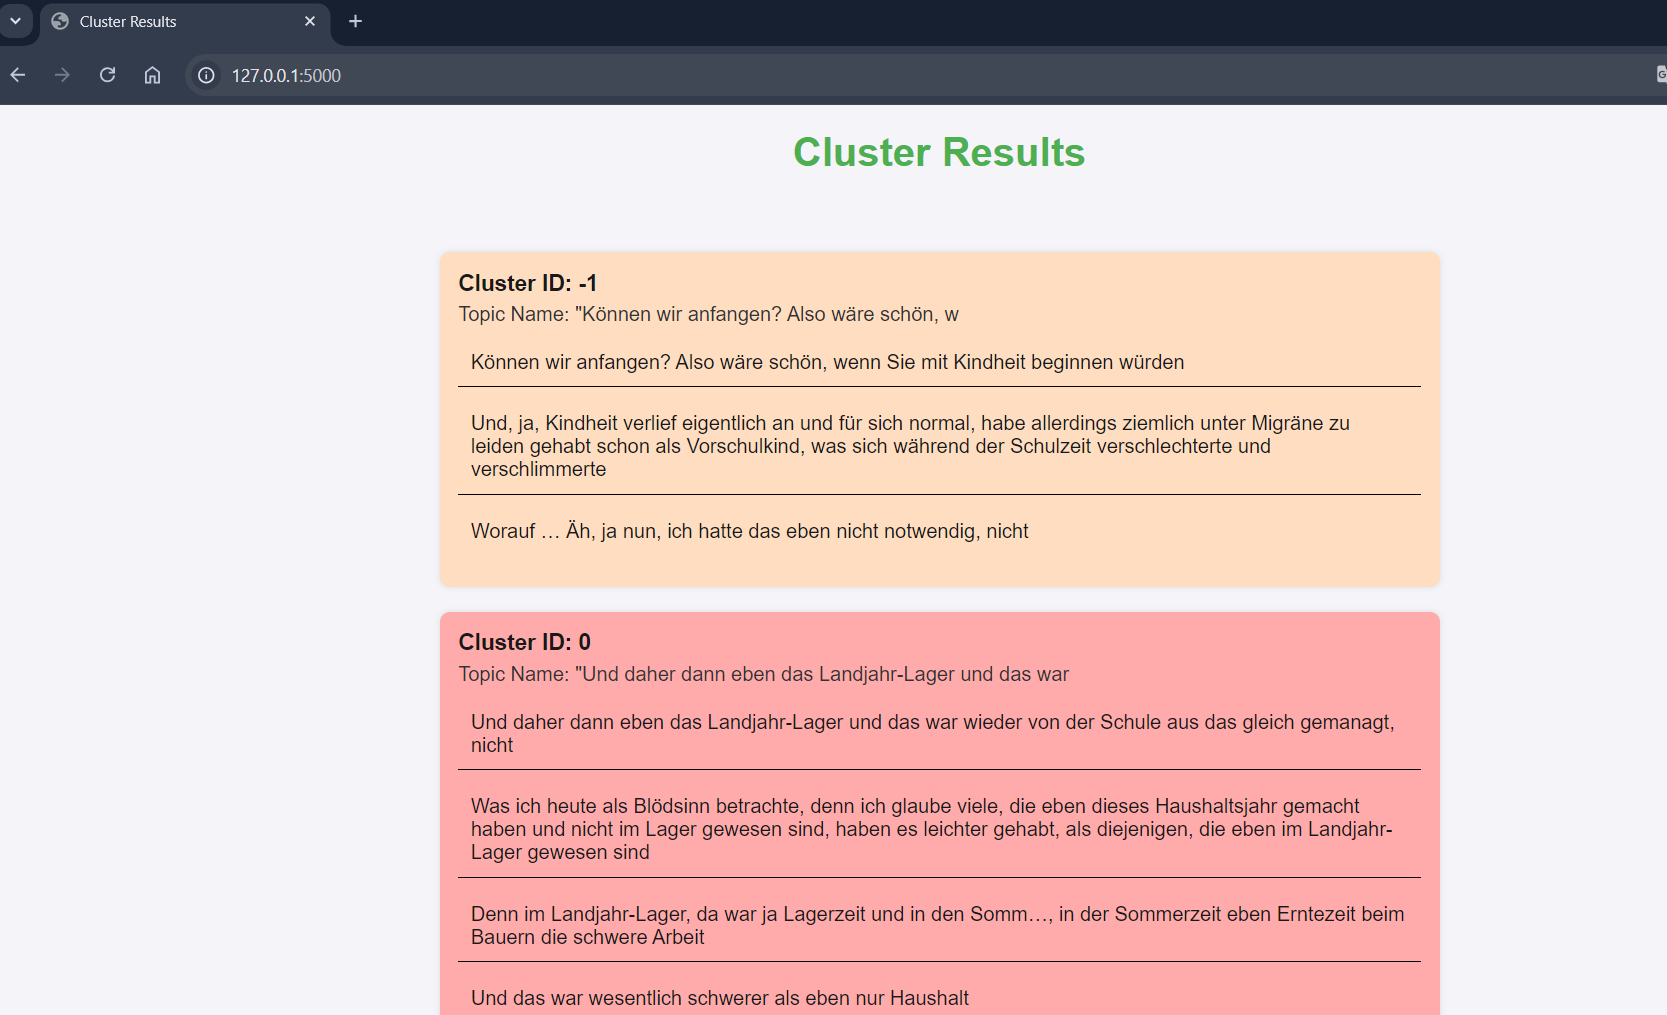
\includegraphics[width=12cm]{./Images/UI Result.png}
       \caption{UI for the web application}
       \label{fig: Web application Output UI}
    \end{center}
\end{figure}


This web application is used to process the smaller text data and generate the topic in the same way as the previous section.
This will help the user to process the data faster and can be used for both German and English language.


\section{Summary}
This chapter gives the detailed explaination about the various libraries used for the implementation of the topic modelling and along with the web application for 
smaller text corpus. The process of achieve the topic modelling on the historical biographical interview data using the embedding, clustering and large language 
model is explained in the previous section. The web application is used to process the smaller text data and generate the topic in the same way as the previous section.
With the help of this implementation approach for achieving topic modelling describe how LLMs can be used for topic modelling when the dealing with the larger text documents.
With this chapter implementation of the thesis is completed and next chapter will be about checking the performance of the models implemented.


